\scanpage{11}

Supposons \deleted{\unsure{tjrs}} que $k$ soit une $\mathbb Q$-algèbre.
\deleted{Alors} Soit $\unsure{\pi(U)|P(U)}$
\deleted{$\unsure{\exp\xi}$} l'ens des éléments primitifs de $U$.
Alors
\deleted{\diagram{\begin{tikzcd}[ampersand replacement=\&]
\unsure{P(U)} \arrow[r] \& \unsure{G}
\end{tikzcd}}}
\diagram{\begin{tikzcd}[ampersand replacement=\&]
\pi(U) \arrow[r,bend left=15,"\exp"] \& \gamma(U) \arrow[l,bend left=15,"\log"]
\end{tikzcd}}
sont des \uline{bijections} \uline{inverses} \uline{l'une de l'autre}.

[N.B. il suffit de vérifier que exp.
applique $\pi(U)$ dans $\gamma(U)$, et log. applique
$\gamma(U)$ dans $\pi(U)$]. \uline{\unsure{Par transport de structure}},
\uline{on obtient sur} $\pi(U)$ une loi \uline{de groupe}. Elle est
donnée à l'aide du crochet, par une formule
\uline{universelle} [\unsure{formule de Campbell} \unsure{et Hausdorff}].
\margin{\uline{\unsure{f\textsuperscript{o} bell-Hausdorff}}, et coefficients des
\unsure{Séries}\unsure{---}\unsure{Exponentielle|Exponentielles}.}

\figure{\begin{tikzpicture}\node[draw,ellipse,inner sep=3pt]{3};\end{tikzpicture}}
Soit $U$ une $k$-\deleted{hyperalgèbre}
\deleted{\unsure{algèbre}} \inserted{algèbre}
\unsure{discrète} \deleted{\unsure{(i.e. séparée)}}
\deleted{\unsure{supp. que} \unsure{)}
\unsure{Alors on prend les élts|Alors on peut les exp} \unsure{)}
\unsure{et} $I(U)$ \unsure{ne soit pas nilpotent, et
exp( ) n'est pas défini a priori}}, soit
$\Lambda$ une $k$-algèbre infinitésimale.
Alors \deleted{$\unsure{K\otimes_k}$} $U\otimes_k\Lambda$ est une
$\Lambda$-hyperalgèbre augmentée ;
\deleted{\unsure{et on a là un autre} \unsure{de} l'idéal
d'augmentation $I(U)\otimes_k\Lambda$
\unsure{n'est pas nilpotent, mais on a}}
\figure{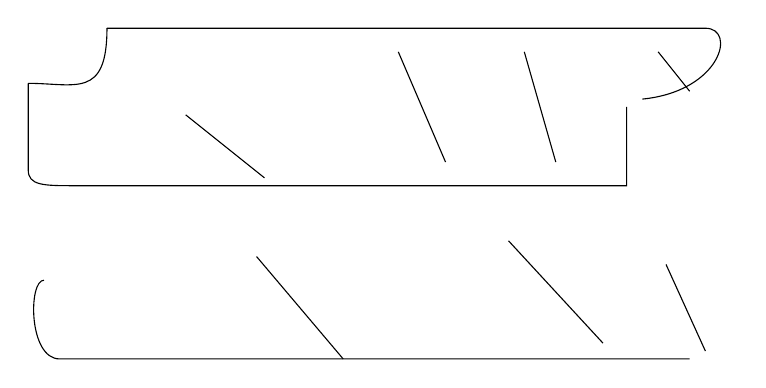
\begin{tikzpicture}[x=1cm,y=1cm]
\draw (1,4.8)--(8.6,4.8) .. controls (9,4.8) and (8.8,4) .. (7.8,3.9);
\draw (1,4.8) .. controls (1,3.9) and (.6,4.1) .. (0,4.1);
\draw (0,4.1)--(0,3) .. controls (0,2.8) and (.2,2.8) .. (.6,2.8)--(7.6,2.8)--(7.6,3.8);
\draw (2,3.7)--(3,2.9) (4.7,4.5)--(5.3,3.1) (6.3,4.5)--(6.7,3.1) (8,4.5)--(8.4,4);
\draw (.2,1.6) .. controls (0,1.6) and (0,.6) .. (.4,.6)--(8.4,.6);
\draw (2.9,1.9)--(4,.6) (6.1,2.1)--(7.3,.8) (8.1,1.8)--(8.6,.7);
\end{tikzpicture}}

\mspage{10}
